\chapter{\MakeUppercase{Fundamentação Teórica}}

A atividade de desenvolvimento de \textit{software} envolve o uso de linguagens de programação, bibliotecas, \textit{frameworks} e metodologias de trabalho para produzir, testar e entregar sistemas. Neste capítulo são apresentados os conceitos e tecnologias que fundamentaram as atividades realizadas durante o estágio, abrangendo o contexto do agronegócio, a metodologia ágil \textit{Scrum} e as tecnologias de desenvolvimento \textit{front-end} utilizadas na construção da plataforma.

\section{Gestão de Dados no Agronegócio}

O agronegócio brasileiro é responsável por uma parcela significativa do Produto Interno Bruto nacional. De acordo com dados do Centro de Estudos Avançados em Economia Aplicada (Cepea), em parceria com a Confederação da Agricultura e Pecuária do Brasil (CNA), o setor tem apresentado crescimento consistente nas últimas décadas, consolidando o país como um dos maiores produtores e exportadores de alimentos do mundo \cite{CepeaCNA2025}.

Nesse contexto, a pesquisa agrícola desempenha papel fundamental para a manutenção e o aumento da produtividade. Instituições e empresas especializadas em análise de solos e sementes coletam grandes volumes de dados ao longo das safras, incluindo informações sobre composição do solo, tratamentos aplicados, condições climáticas e resultados de produtividade. Tradicionalmente, esses dados são registrados em planilhas eletrônicas e documentos avulsos, o que dificulta a rastreabilidade, a padronização e a análise integrada das informações \cite{Embrapa2019}.

Com o avanço da chamada Agricultura 4.0, a digitalização dos processos agrícolas tornou-se uma tendência crescente. A Agricultura 4.0 é caracterizada pela adoção de tecnologias digitais, como sensores, \textit{Internet das Coisas} (IoT), computação em nuvem e análise de dados, com o objetivo de otimizar a tomada de decisões no campo \cite{Massruha2020}. Nesse cenário, plataformas \textit{web} que centralizam o registro e a análise de dados de pesquisa representam uma evolução em relação ao uso descentralizado de planilhas, permitindo que os colaboradores acessem informações atualizadas, apliquem regras de negócio padronizadas e gerem visualizações gráficas de forma automatizada.

\section{Metodologias Ágeis: O \textit{Framework Scrum}}

O \textit{Scrum} é um \textit{framework} de gerenciamento de projetos e desenvolvimento ágil com formato iterativo e incremental. Cada ciclo no \textit{Scrum} é conhecido como \textit{Sprint}, um processo com duração de tempo fixa e com um conjunto de tarefas que devem ser implementadas nesse período. No final de cada \textit{Sprint}, uma nova versão com novas funcionalidades e melhorias do sistema é entregue \cite{Schwaber2020}.

No \textit{Scrum}, antes do início de uma \textit{Sprint}, ocorre uma reunião de planejamento chamada \textit{planning}. Nela, o \textit{Product Owner} seleciona as tarefas do \textit{Product Backlog}, que é a lista priorizada com todas as funcionalidades e melhorias planejadas para o produto, e as adiciona ao \textit{Sprint Backlog}, definindo o escopo de trabalho da \textit{Sprint}. O \textit{Product Owner} é o responsável por definir a prioridade das tarefas e planejar o lançamento de novas funcionalidades.

Outra figura-chave no processo do \textit{Scrum} é o \textit{Scrum Master}, pessoa responsável por garantir que os conceitos da metodologia estão sendo aplicados de maneira correta e por remover impedimentos que possam atrapalhar o progresso da equipe. A equipe de desenvolvimento, por sua vez, é composta pelos profissionais que efetivamente executam as tarefas planejadas.

Além da \textit{planning}, o \textit{Scrum} prevê reuniões diárias chamadas \textit{daily meetings}, nas quais cada membro da equipe compartilha o que foi feito no dia anterior, o que será feito no dia atual e se há algum impedimento. No final da \textit{Sprint}, ocorrem a \textit{Sprint Review}, na qual o incremento do produto é apresentado, e a \textit{Sprint Retrospective}, na qual a equipe discute o que funcionou bem e o que pode ser melhorado no processo.

No projeto desenvolvido durante o estágio na Zeeway, o \textit{Scrum} foi adotado como metodologia de desenvolvimento, com \textit{Sprints} de duração fixa, reuniões de planejamento e acompanhamento por meio de \textit{dailies}. A adoção dessa metodologia permitiu entregas incrementais ao cliente e uma organização clara das tarefas ao longo do projeto.

\section{Tecnologias de Desenvolvimento \textit{Front-end}}

Nesta seção são apresentadas as principais tecnologias utilizadas no desenvolvimento da interface da plataforma de protocolos. A escolha dessas tecnologias levou em consideração a necessidade de construir uma aplicação \textit{web} interativa, com formulários complexos, tabelas dinâmicas e visualizações gráficas.

\subsection{React e TypeScript}

O \textit{React} é uma biblioteca \textit{JavaScript} de código aberto, criada pelo \textit{Facebook} (atualmente \textit{Meta}), voltada para a construção de interfaces de usuário. Seu principal conceito é a componentização: a interface é dividida em componentes reutilizáveis, cada um responsável por renderizar uma parte específica da tela. Os componentes podem receber dados por meio de propriedades (\textit{props}) e gerenciar seu próprio estado interno utilizando \textit{hooks} como \texttt{useState} e \texttt{useEffect} \cite{React2024}.

Uma das vantagens do \textit{React} é o uso do \textit{Virtual DOM} (\textit{Document Object Model}), uma representação virtual da árvore de elementos da página. Quando o estado de um componente é alterado, o \textit{React} compara a versão atual do \textit{Virtual DOM} com a anterior e atualiza apenas os elementos que de fato mudaram, otimizando a performance de renderização.

O \textit{TypeScript} é um superconjunto do \textit{JavaScript} desenvolvido pela \textit{Microsoft} que adiciona tipagem estática à linguagem. Em projetos \textit{React}, o \textit{TypeScript} permite definir tipos para as \textit{props} dos componentes, para os dados recebidos de APIs e para o estado da aplicação, reduzindo erros em tempo de desenvolvimento e facilitando a manutenção do código \cite{TypeScript2024}. O \autoref{cod:reactts} apresenta um exemplo didático de um componente React escrito em TypeScript.

\begin{lstlisting}[caption={Exemplo didático de um componente \textit{React} com \textit{TypeScript}.}, label={cod:reactts}]
import { useState } from "react";

interface ContadorProps {
  inicial: number;
  passo?: number;
}

export function Contador({ inicial, passo = 1 }: ContadorProps) {
  const [valor, setValor] = useState<number>(inicial);

  return (
    <button onClick={() => setValor(valor + passo)}>
      Cliques: {valor}
    </button>
  );
}
\end{lstlisting}

No exemplo, a interface \texttt{ContadorProps} declara as propriedades aceitas pelo componente, indicando que \texttt{inicial} é obrigatória e que \texttt{passo} é opcional (sinalizada pela interrogação) com valor padrão igual a um. O componente \texttt{Contador} recebe essas propriedades já tipadas, mantém um estado interno por meio do \textit{hook} \texttt{useState} (cuja tipagem também é explícita) e retorna um elemento de interface (botão) cujo clique incrementa o valor do estado, fazendo com que o \textit{React} reexecute a função e atualize a tela com o novo valor.

No projeto da plataforma de protocolos, a combinação de \textit{React} com \textit{TypeScript} foi utilizada para construir todos os componentes da interface. A ferramenta de \textit{build} adotada foi o \textit{Vite}, que oferece um servidor de desenvolvimento com \textit{Hot Module Replacement} (HMR), permitindo que as alterações no código fossem refletidas instantaneamente no navegador durante o desenvolvimento.

\subsection{Gerenciamento de Estado e Formulários}

Em aplicações \textit{React} de maior porte, o gerenciamento do estado da aplicação torna-se um desafio. Para solucionar esse problema, foi utilizada a biblioteca \textit{Zustand}, uma solução leve de gerenciamento de estado global que permite compartilhar dados entre componentes sem a necessidade de passar \textit{props} por múltiplos níveis da árvore de componentes \cite{Zustand2024}. Em conjunto com o \textit{Zustand}, foram empregados o seu \textit{middleware} de persistência, para manter a sessão do usuário entre acessos, e a biblioteca \textit{Immer}, que permite atualizar o estado de forma imutável por meio de uma sintaxe direta. A biblioteca \textit{jwt-decode} foi utilizada para decodificar o \textit{token} JWT recebido no login e extrair as informações do usuário.

Para o gerenciamento dos formulários, que constituíam uma parte central da plataforma dado o grande número de campos nos protocolos, foram utilizadas as bibliotecas \textit{Formik} e \textit{Yup}. O \textit{Formik} é uma biblioteca que simplifica a criação de formulários em \textit{React}, cuidando do estado dos campos, da validação e do envio dos dados. O \textit{Yup} é uma biblioteca de validação de esquemas que permite definir regras de validação de forma declarativa, como campos obrigatórios, tipos de dados esperados e validações condicionais \cite{Formik2024}. O \autoref{cod:yupex} apresenta um exemplo didático de um esquema de validação com \textit{Yup}.

\begin{lstlisting}[caption={Exemplo didático de um esquema de validação com \textit{Yup}.}, label={cod:yupex}]
import * as Yup from "yup";

const esquemaUsuario = Yup.object().shape({
  nome: Yup.string().required("Nome obrigatorio"),
  email: Yup.string().email("E-mail invalido").required("E-mail obrigatorio"),
  idade: Yup.number().min(18, "Idade minima 18").nullable(),
});
\end{lstlisting}

No exemplo, \texttt{Yup.object().shape} declara o formato esperado de um objeto. Cada chave do objeto encadeia validações específicas: \texttt{nome} deve ser uma \textit{string} obrigatória; \texttt{email} deve ter formato válido e ser obrigatório, combinando duas regras na mesma cadeia; \texttt{idade} deve ser um número de pelo menos dezoito, mas pode receber valor nulo. A mensagem passada a cada validação é o texto exibido ao usuário quando a regra é violada.

A comunicação com a API do servidor foi implementada por meio da biblioteca \textit{Axios}, um cliente HTTP que permite realizar requisições de forma simplificada. Para o gerenciamento de cache e sincronização dos dados do servidor, foi utilizada a biblioteca \textit{React Query} (\textit{TanStack Query}), que automatiza o processo de busca, cache, atualização e invalidação de dados, evitando requisições desnecessárias e mantendo a interface atualizada \cite{TanStackQuery2024}.

\subsection{Design de Interface com Material UI (MUI)}

O \textit{Material UI} (MUI) é uma biblioteca de componentes \textit{React} que implementa o \textit{Material Design}, sistema de design criado pelo \textit{Google}. A biblioteca fornece um conjunto amplo de componentes prontos, como botões, campos de texto, tabelas, menus, modais e \textit{date pickers}, todos com aparência e comportamento consistentes \cite{MUI2024}. A \autoref{fig:mui} apresenta um exemplo de aplicação construída com o \textit{Material UI}, divulgado pela própria biblioteca, em que diferentes componentes (menu lateral, \textit{cards} de métricas, gráficos e tabelas) são combinados de forma coesa.

\begin{figure}[!htb]
\centering
\caption{Exemplo de aplicação construída com o \textit{Material UI}.}
\label{fig:mui}
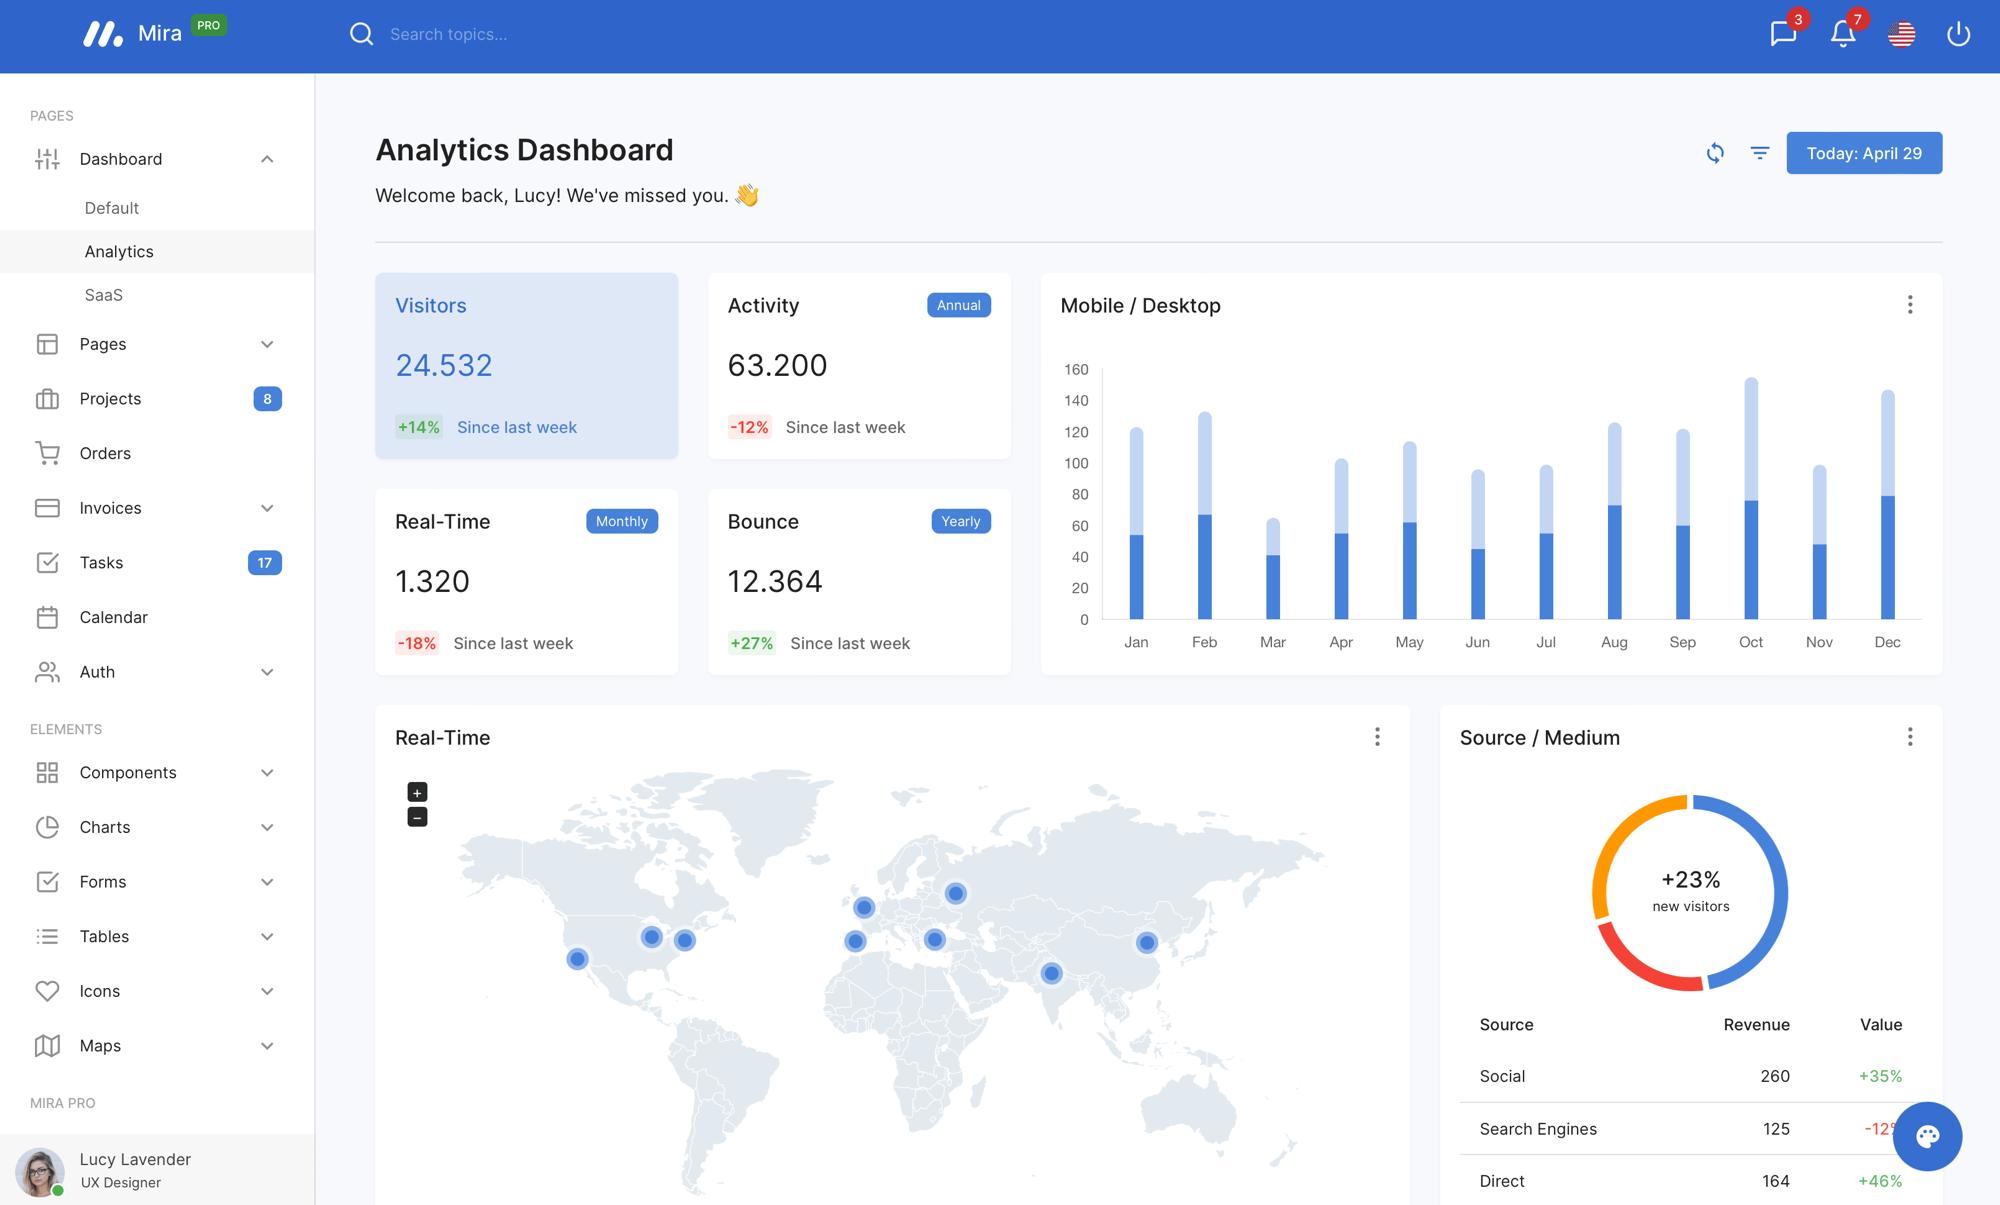
\includegraphics[width=0.90\textwidth,height=0.45\textheight,keepaspectratio]{imgs/mui_dashboard.png}
\fonte{Material UI. Disponível em: https://mui.com/. Acesso em: maio 2026.}
\end{figure}

Uma das vantagens do \textit{MUI} é a possibilidade de personalização por meio de temas. No projeto desenvolvido durante o estágio, foi criado um tema personalizado que definia as cores, tipografia e espaçamentos de acordo com a identidade visual da empresa cliente. Dessa forma, todos os componentes da biblioteca adotavam automaticamente o padrão visual definido, garantindo consistência em toda a plataforma.

Além dos componentes básicos do \textit{MUI}, o projeto utilizou a biblioteca \textit{MUI X Date Pickers} para os campos de seleção de data, recurso frequentemente utilizado nos formulários de protocolos que exigiam o registro de datas de plantio, colheita e emergência. Também foi utilizada a biblioteca \textit{TanStack React Table} para a construção de tabelas com funcionalidades avançadas de ordenação, paginação e filtragem.

\subsection{Visualização de Dados com ApexCharts}

A geração de gráficos e visualizações de dados constituiu o principal diferencial da plataforma em relação ao uso de planilhas. Para essa funcionalidade, foi utilizada a biblioteca \textit{ApexCharts}, uma biblioteca \textit{JavaScript} de código aberto para a criação de gráficos interativos. A integração com o \textit{React} foi realizada por meio do pacote \textit{react-apexcharts} \cite{ApexCharts2024}.

O \textit{ApexCharts} oferece diversos tipos de gráficos, como barras, linhas, pizza, radar e área, além de funcionalidades como \textit{zoom}, \textit{tooltip} e exportação em formato de imagem. Na plataforma de protocolos, foram utilizados principalmente gráficos de barras verticais e horizontais para comparar os resultados entre diferentes tratamentos e momentos de avaliação. O \autoref{cod:apexex} apresenta um exemplo didático da configuração mínima de um gráfico de barras com o pacote \textit{react-apexcharts}.

\begin{lstlisting}[caption={Exemplo didático de gráfico de barras com \textit{react-apexcharts}.}, label={cod:apexex}]
import ApexCharts from "react-apexcharts";

const series = [{ name: "Vendas", data: [10, 20, 30] }];
const options = {
  chart: { type: "bar" },
  xaxis: { categories: ["Jan", "Fev", "Mar"] },
};

export function GraficoVendas() {
  return <ApexCharts options={options} series={series} type="bar" />;
}
\end{lstlisting}

No exemplo, \texttt{series} é a lista de séries do gráfico, cada uma contendo um nome e um vetor de valores numéricos correspondentes a cada categoria. O objeto \texttt{options} concentra a configuração visual, definindo o tipo de gráfico (\texttt{chart.type}) e os rótulos do eixo horizontal (\texttt{xaxis.categories}). O componente \texttt{ApexCharts} recebe esses dois objetos e cuida da renderização do gráfico na tela.

\novop{A \autoref{fig:apexex} apresenta uma representação aproximada do gráfico produzido pelo \autoref{cod:apexex}, em que as três categorias (Jan, Fev e Mar) são exibidas no eixo horizontal e os valores numéricos correspondentes (10, 20 e 30) compõem as barras verticais.}

\begin{figure}[!htb]
\centering
\caption{\novo{Renderização aproximada do gráfico de barras configurado no \autoref{cod:apexex}.}}
\label{fig:apexex}
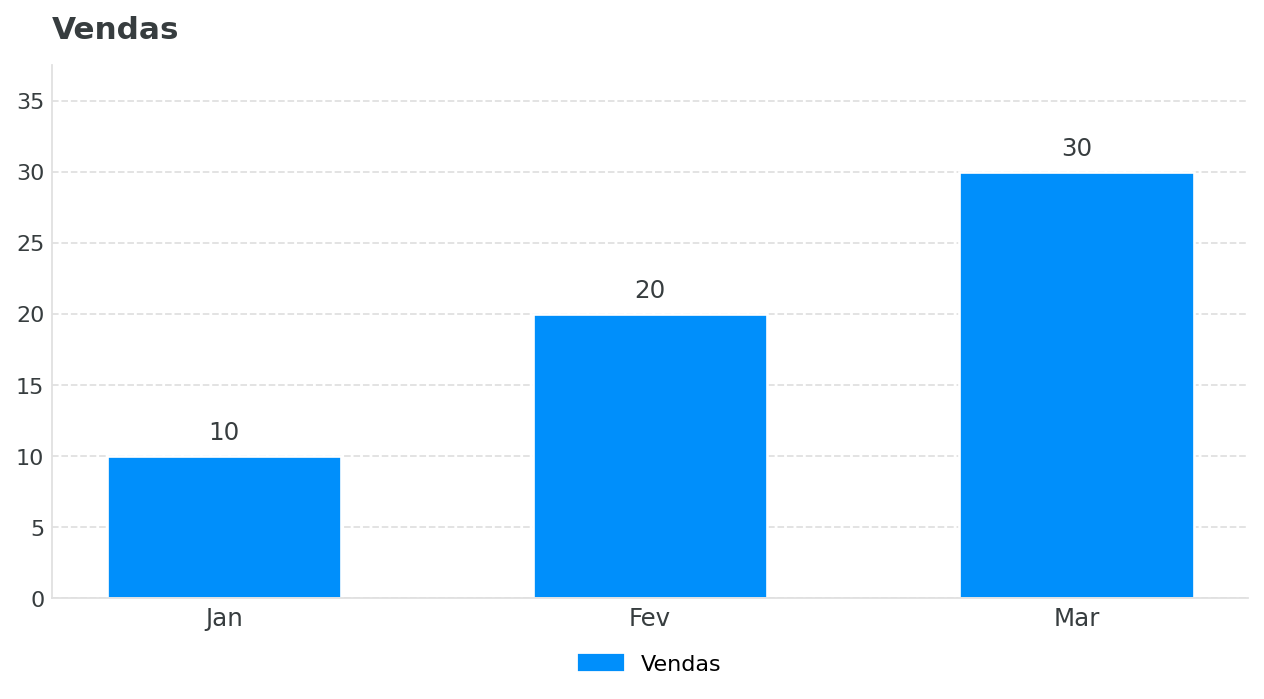
\includegraphics[width=0.65\textwidth,height=0.30\textheight,keepaspectratio]{imgs/apexcharts_vendas.png}
\fonte{\novo{do autor (2026), com base na biblioteca \textit{ApexCharts}.}}
\end{figure}

Para a avaliação de campos definidos como fórmulas nos protocolos, isto é, expressões matemáticas calculadas a partir dos valores de outros campos, foi utilizada a biblioteca \textit{mathjs}, que interpreta e avalia expressões em tempo de execução. A exportação dos gráficos em formato de imagem, com a identidade visual da empresa cliente, foi implementada com a biblioteca \textit{use-react-screenshot}, que captura um elemento da interface como imagem. Já a biblioteca \textit{JSZip} foi empregada para empacotar as fotografias de campo de uma avaliação em um único arquivo compactado para \textit{download}.
